\documentclass[conference]{IEEEtran}
\IEEEoverridecommandlockouts

\usepackage[numbers,sort&compress]{natbib}
\usepackage{tabularx,booktabs}
\usepackage{amsmath,amssymb,amsfonts}
\usepackage{algorithmic}
\usepackage{graphicx}
\usepackage{numprint}
\usepackage{textcomp}
\usepackage{xcolor}
\usepackage{ifthen}
\usepackage{float}
\usepackage[hyphens]{url}
\urlstyle{same}

\usepackage{tikz}
\usetikzlibrary{positioning,chains}
\usepackage{pgfplots}
\pgfplotsset{compat=1.18}

\usepackage [english]{babel}
\usepackage [autostyle, english = american]{csquotes}
\MakeOuterQuote{"}

\newcolumntype{B}{>{\hsize=.6\hsize}X}
\newcolumntype{M}{>{\hsize=.4\hsize}X}
\newcolumntype{s}{>{\hsize=.2\hsize}X}

\newcommand{\lithead}[3][]{
	\textbf{
		\ifthenelse{\equal{#1}{}}{\citeauthor{#2}}{#1}
		(\citeyear{#2})
		\cite{#2}.
	}
	#3
}

\def\BibTeX{{\rm B\kern-.05em{\sc i\kern-.025em b}\kern-.08em
    T\kern-.1667em\lower.7ex\hbox{E}\kern-.125emX}}

\begin{document}
	\bstctlcite{BSTSettings}

	\title{A Survey On AI-Based Clothing Recommendation For Try Before Buy}

	\makeatletter
	\newcommand{\linebreakand}{
		\end{@IEEEauthorhalign}
		\hfill\mbox{}\par
		\mbox{}\hfill\begin{@IEEEauthorhalign}
	}
\makeatother

\author{
	\IEEEauthorblockN{Dr. N K Bansode}
	\IEEEauthorblockA{
		\textit{Dept. of Computer Engineering} \\
		\textit{Army Institue of Technology}\\
		Pune, India \\
		nkbansode@aitpune.edu.in
	}
	\and
	\IEEEauthorblockN{Vipin Kumar Yadav}
	\IEEEauthorblockA{
		\textit{Dept. of Computer Engineering} \\
		\textit{Army Institue of Technology}\\
		Pune, India \\
		vipinkumar\_20204@aitpune.edu.in
	}
	\and
	\IEEEauthorblockN{Risabh Rai}
	\IEEEauthorblockA{
		\textit{Dept. of Computer Engineering} \\
		\textit{Army Institue of Technology}\\
		Pune, India \\
		rishabhrai\_20150@aitpune.edu.in
	}
	\linebreakand
	\IEEEauthorblockN{Uday Bhanu Bose}
	\IEEEauthorblockA{
		\textit{Dept. of Computer Engineering} \\
		\textit{Army Institue of Technology}\\
		Pune, India \\
		udaybose\_20128@aitpune.edu.in
	}
	\and
	\IEEEauthorblockN{Vivek Tiwari}
	\IEEEauthorblockA{
		\textit{Dept. of Computer Engineering} \\
		\textit{Army Institue of Technology}\\
		Pune, India \\
		vivektiwari\_20181@aitpune.edu.in
	}
}

	\maketitle

	
\begin{abstract}
	In the rapidly evolving landscape of fashion e-commerce, the fusion of artificial intelligence (AI) technologies has ushered in a transformative era. This survey paper delves into the pivotal realm of AI-based Clothing Recommendation and Virtual Try-On Systems, discussing their impacts on the fashion industry and consumers alike. Recommendation systems, a cornerstone of personalized shopping experiences, are examined in detail. We explore diverse approaches, from fashion item compatibility to complete outfit generation, highlighting their pivotal role in tailoring clothing suggestions to individual preferences. These systems not only enhance customer satisfaction but also contribute significantly to the growth and sustainability of online fashion businesses. Simultaneously, Virtual Try-On Systems emerge as a revolutionary solution to address the biggest challenge of online clothing shopping - "Will it fit and look good on me?"
	
	Our analysis spans various dimensions of virtual try-on, including everything from 2D image-based systems to cutting-edge AR solutions. By virtually placing customers in garments, these systems offer an immersive, confidence-boosting experience, ultimately reducing return rates and enhancing overall customer trust. This literature review provides a comprehensive analysis of the current state of clothing recommendation and virtual try-on systems, with a particular focus on their integration of artificial intelligence and machine learning, computer vision, and augmented reality (AR). Computer vision techniques have enabled accurate garment recognition, facilitating virtual try-on experiences that bridge the gap between online and offline shopping. AR further elevates user engagement by enabling consumers to virtually "try on" clothing items in real-time.
	
	As we explore the technologies and practical implementations, we shed light on the remarkable strides made in the fashion industry, empowering customers to make informed and satisfying clothing choices in the digital realm.
\end{abstract}

\begin{IEEEkeywords}
	artificial intelligence, augmented reality, clothing recommendation, computer vision, virtual try-on
\end{IEEEkeywords}

	\section{Introduction} \label{section:intro}
	In today's fast-paced world, the biggest appeal of e-commerce is the ability to view and purchase items from a large catalog without having to physically visit the store. Getting items delivered to the doorstep is convenient because it saves time and mental overhead on many levels. However, while this is true for most items, the fashion industry is still lagging behind.

	The online fashion retail market sees return rates of as high as 50\% with "did not fit", "did not like", and "planned product return (show-rooming)" as some of the main cited reasons \cite{stocker2021new}.

	The two solutions to this problem are good recommendation systems which suggest clothing that look good on the consumer and aligns with their preferences, and virtual try-on systems that eliminate the need to buy a selection of items only to return most of them.

	This survey paper explores the field of clothing recommendation and virtual try-on systems, shedding light on their evolving capabilities and significant impact on the e-commerce ecosystem. In this exploration of the state of these technologies, we delve into the underlying methodologies, recent breakthroughs, and the multitude of applications across various e-commerce platforms. As we navigate this survey, we uncover the pivotal role these systems play in shaping the future of fashion retail, fostering more informed and immersive shopping experiences for consumers worldwide.

	Previous surveys have provided a comprehensive list of techniques and technologies available in the space, going into details of how computer vision was being used for fashion detection, analysis, and synthesis \cite{DBLP:journals/csur/ChengSCHL21, Jain_Wah_2022}, how modern recommender systems work \cite{DBLP:journals/corr/abs-2202-02757, DBLP:journals/sncs/ShirkhaniMSH23}, the state of virtual try-on systems \cite{DBLP:journals/corr/abs-2111-00905, DBLP:journals/mta/GhodhbaniNRA22, DBLP:journals/cvm/LiangL21}, the use, impact, and challenges of augmented reality in the fashion industry \cite{menon2020impact, jayamini2021use, DBLP:journals/corr/abs-2202-09450, huang2019enhancing, mehta2020enhancement, zak2020augmented, caboni2019augmented}, and the general use of AI in fashion design and commerce \cite{DBLP:journals/access/GiriJZB19, DBLP:journals/corr/abs-2105-03050, DBLP:journals/access/GuoZLCCW23, DBLP:journals/spm/ChenSC23, sahni2021review, liang2020implementation, sareen2022ai, 10153335, DBLP:journals/tmm/Yan0LZX0Y23}.

	The survey is structured as follows: Section \ref{section:survey-methodology} describes the methodology behind the survey. Section \ref{section:rs} is dedicated to recommendation systems, where we discuss the techniques used and provide a comparative analysis of the research in the field. In Section \ref{section:vton}, we explore virtual try-on systems, where we go over the prominent work done in the area. In Section \ref{section:datasets} we list and discuss the various datasets available for use in the domain. And finally, we conclude in Sections \ref{section:conclusion} and \ref{section:future}.
	\section{Survey Methodology and Results} \label{section:survey-methodology}
	\subsection{Research Design}
		This review is based on a systematic survey of studies primarily done within the period 2019 to 2023. Most recent information has been included for advancement in the field of fashion recommendation and virtual try-on.
	
	\subsection{Search Strategy}
		\textit{Google Scholar} and the \textit{dblp computer science bibliography} have been instrumental in providing results for searches using important keywords like, `artificial intelligence, augmented reality, clothing, fashion, recommendation, computer vision, and virtual try-on.'

	\subsection{Inclusion \& Exclusion Criteria}
		The survey was conducted with the following inclusion criteria:
		\begin{enumerate}
			\item Does the study deal with the use of technologies in fashion for recommenders and virtual try-on?
			\item Is the study comparable to existing state-of-the-art techniques?
		\end{enumerate}
	
	\subsection{Survey Results}
		147 documents were included in the final collection for analysis. Figure \ref{fig:document-collection} illustrates the flow of the collection process, and Figure \ref{fig:document-domains} shows the distribution of the collected documents per domain.

	\begin{figure}
		\centering
		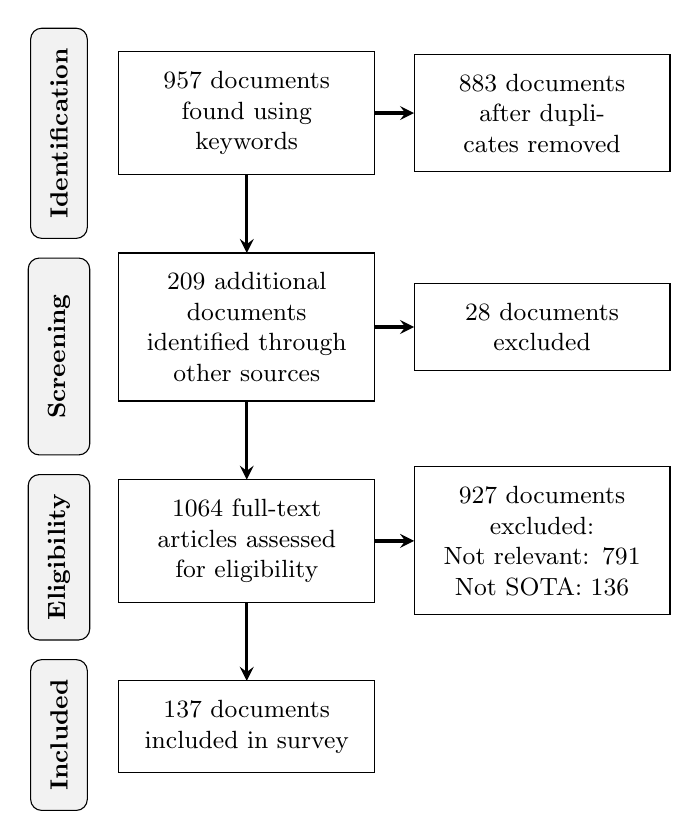
\begin{tikzpicture}[
			node distance=10mm and 5mm,
			start chain=going below,
			rNode/.style = {
				draw, rectangle, align=center, text width=2.75cm,
				font=\small, inner sep=2.5mm, outer sep=0pt,
				on chain},
			mylabel/.style = {
				draw, rectangle, align=center, rounded corners, 
				font=\small\bfseries, inner sep=2.5mm, outer sep=0pt,
				fill=black!5, minimum height=30mm,
				on chain},
			every join/.style = arrow,
			arrow/.style = {very thick,-stealth}
		]
			\node (n1) [rNode] {957 documents found using keywords};
			\node (n2) [rNode, join] {209 additional documents identified  through other sources};
			\node (n3) [rNode, join] {1064 full-text articles assessed for eligibility};
			\node (n4) [rNode, join] {137 documents included in survey};
			\node (n1r) [rNode, right=of n1] {883 documents after duplicates removed};
			\node (n2r) [rNode, right=of n2] {28 documents excluded};
			\node (n3r) [rNode, right=of n3] {927 documents excluded:\\
				Not relevant: 791 \\
				Not SOTA: 136
			};
			\draw[arrow] (n1) -- (n1r);
			\draw[arrow] (n2) -- (n2r);
			\draw[arrow] (n3) -- (n3r);
			\begin{scope}[node distance=2.5mm]
				\node[mylabel,below left=-3mm and 4mm of n1.north west, minimum height=20mm] {\rotatebox{90}{Identification}};
				\node[mylabel, minimum height=25mm] {\rotatebox{90}{Screening}};
				\node[mylabel, minimum height=21mm] {\rotatebox{90}{Eligibility}};
				\node[mylabel, minimum height=19mm] {\rotatebox{90}{Included}};
			\end{scope}
		\end{tikzpicture}
		\caption{Document collection flowchart}
		\label{fig:document-collection}
	\end{figure}

	\begin{figure}
		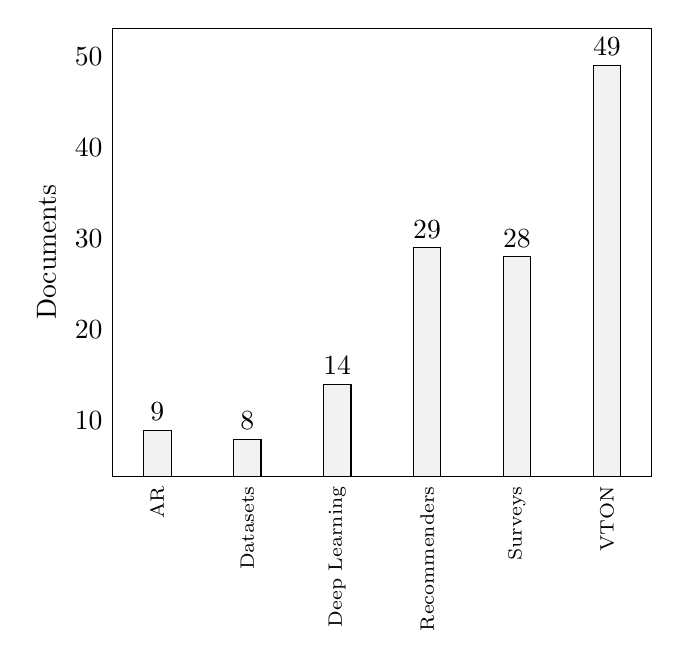
\begin{tikzpicture}
			\begin{axis}[
				symbolic x coords={AR, Datasets, Deep Learning, Recommenders, Surveys, VTON},
				ylabel = {Documents},
				xticklabel style = {font=\scriptsize, anchor=east, rotate=90},
				xtick=data,
				nodes near coords,
				tick style={draw=none}
			]
				\addplot[ybar, fill=black!5] coordinates {
					(AR, 9)
					(Datasets, 8)
					(Deep Learning, 14)
					(Recommenders, 29)
					(Surveys, 28)
					(VTON, 49)
				};
			\end{axis}
		\end{tikzpicture}
		\caption{Document domain distribution}
		\label{fig:document-domains}
	\end{figure}

	% Total papers:

	% Fashion (957)
	% 	2023 (155)
	% 	2022 (211)
	% 	2021 (193)
	% 	2020 (190)
	% 	2019 (208)
	% Recommenders (116)
	% 	2023 (13)
	% 	2022 (29)
	% 	2021 (18)
	% 	2020 (21)
	% 	2019 (35)
	% VTON (200)
	% 	2023 (36)
	% 	2022 (66)
	% 	2021 (49)
	% 	2020 (22)
	% 	2019 (27)
	\section{Recommendation systems} \label{section:rs}
	Recommendation systems leverage data and algorithms to offer personalized suggestions to users, enhancing their decision-making in various domains. These systems use collaborative filtering, content-based filtering, and hybrid approaches, facilitating tailored content, product, or service recommendations, ultimately improving user engagement and satisfaction in diverse applications, from e-commerce to content streaming.

	Clothing and fashion recommendation systems present a unique and intricate challenge compared to general recommendation systems. They must consider not only user preferences but also the highly subjective and context-dependent nature of fashion. Recommending apparel necessitates understanding intricate details like style, fit, and individual tastes, which can evolve over time. The ever-changing fashion trends further complicate the task. Fashion items often involve combinations, making recommendations more complex.

	Moreover, the emotional aspect of fashion and the need for users to express their individuality make it challenging to predict preferences accurately. These systems must encompass visual recognition, trend analysis, and personalization, making fashion recommendation systems not only distinct but also more demanding to develop with precision.

	\subsection{Goals of recommendation systems}
		Studying the literature for clothing and fashion recommendation systems reveals the following goals:

		\begin{enumerate}
			\item \textbf{Outfit recommendation:} This is similar to the goal of generic recommendation systems as it aims to recommend garments or outfits based on the user's preferences (e.g., complex color patterns, or specific fabrics and textures), body attributes like color and shape, current trends, and custom contexts specified by the user (e.g., outfit for a formal party) \cite{DBLP:conf/sigir/LiW0CXC20, 9156794, 8932738, DBLP:conf/mm/HidayatiHCHFC18, DBLP:journals/tmm/ZhangJGZZLT17, DBLP:conf/waim/ShaWZFZY16}.
			
			\item \textbf{Outfit generation:} This goal is, given a clothing item (e.g., a shirt), find the best garment (e.g., a tie) or outfit (e.g., from pants, skirts, ties, shoes, or hats) that is compatible with the given item. A special case of this goal is pair generation, where one item is the query and a suitable pairing item is needed. This is usually done for top and bottom items \cite{9156535, 9893574, DBLP:conf/kdd/ChenHXGGSLPZZ19}.
			
			\item \textbf{Outfit completion:} This is when most of the outfit is in place, and the task is to complete the outfit's missing items (e.g., what shoes to wear with this outfit?). Also known as fill-in-the-blank (FITB) test \cite{9857004, DBLP:journals/corr/abs-2005-06584, DBLP:conf/mm/SongHLCXN19}.
			
			\item \textbf{Outfit compatibility evaluation:} Also an implicit goal for other tasks, this aims to score an outfit based on how compatible its constituent elements are. This can be used as a metric to rank outfits (e.g., does the red shirt go well with the black skirt and black socks or is the white shirt better?) \cite{DBLP:journals/eswa/MoZPW23, 10049142, DBLP:journals/eswa/BalimO23,9775146, DBLP:conf/iccvw/KimSMSSP21, DBLP:journals/ijon/SunHWZP20, DBLP:conf/sigir/DongWSDN20, DBLP:conf/www/YinL0019, DBLP:conf/aaai/YangMLWC19}.

			\item \textbf{Explainable recommendation:} An explanation clarifies why something was recommended to the user. Explanations are more transparent than black-box recommendations and improve the user experience in a variety of ways. They enhance user trust and understanding, lead to error detection and correction, mitigate bias and promote fairness, and increase user engagement. In recent years, more work has been done on explainable fashion recommendation \cite{DBLP:journals/tomccap/YangSFWDN21, DBLP:journals/www/LiCH21, 9522737, DBLP:journals/tkde/LinRCRMR20, DBLP:conf/wacv/TangsengO20, DBLP:conf/ijcai/HouWCLZL19, DBLP:conf/sigir/ChenCXZ0QZ19}.
		\end{enumerate}
	
		\newcommand{\checkif}[1]{
			\ifthenelse{\equal{#1}{Y}}{\checkmark}{}
		}
		\newcommand{\rsrow}[8]{
			\citeauthor{#1} \cite{#1} & \citeyear{#1} & #2 &
			\checkif{#3} &
			\checkif{#4} &
			\checkif{#5} &
			\checkif{#6} &
			\checkif{#7} &
			\checkif{#8}
			\\
		}
		
		\begin{table*}
			\caption{Recommendation Systems}
			\label{table:rs}
			\begin{tabularx}{\textwidth}{
				p{2.8cm} p{0.5cm} X |
				>{\centering\arraybackslash}p{0.6cm} 
				>{\centering\arraybackslash}p{1.4cm} |
				>{\centering\arraybackslash}p{0.75cm}
				>{\centering\arraybackslash}p{0.6cm}
				>{\centering\arraybackslash}p{1.3cm} |
				>{\centering\arraybackslash}p{1.5cm}
			}
				\toprule
					\textbf{Authors} &
					\textbf{Year} &
					\textbf{Technique(s)} &
					\multicolumn{2}{c|}{\textbf{User Inputs}} &
					\multicolumn{3}{c|}{\textbf{Outputs}} &
					\textbf{Personalized}
					\\
					& & &
					Body Attr. & Interactions\footnotemark[1] &
					Compat. & Outfit Gen. & Explainable
					& \\
				\midrule
					\rsrow{DBLP:journals/eswa/MoZPW23}{
						Transformer $\rightarrow$ Transformer
					}{Y}{}{Y}{Y}{}{Y}
					\rsrow{10049142}{
						Contextual Attention Network
					}{}{}{Y}{Y}{}{}
					\rsrow{DBLP:journals/eswa/BalimO23}{
						CNN $\rightarrow$ LSTM + Transformer
					}{}{Y}{Y}{}{Y}{}
					\rsrow{9857004}{
						Triplet Network
					}{}{}{Y}{Y}{}{}
					\rsrow{9893574}{
						Bi-LSTM, GAN
					}{}{}{Y}{Y}{}{}
					\rsrow{9775146}{
						Bi-LSTM
					}{}{}{Y}{Y}{}{}
					\rsrow{DBLP:journals/tomccap/YangSFWDN21}{
						Representation Learning
					}{}{Y}{Y}{Y}{Y}{}
					\rsrow{DBLP:conf/iccvw/KimSMSSP21}{
						CNN + Projection Head
					}{}{}{Y}{Y}{}{}
					\rsrow{9156535}{
						CNN + Triplet Network
					}{}{}{Y}{Y}{}{}
					\rsrow{DBLP:conf/sigir/DongWSDN20}{
						Bi-LSTM
					}{}{}{Y}{Y}{}{}
					\rsrow{DBLP:journals/ijon/SunHWZP20}{
						LSTM + Triplet Network
					}{}{}{Y}{Y}{}{}
					\rsrow{9156794}{
						CNN + SMPL Est. $\rightarrow$ Joint Embedding
					}{Y}{}{Y}{Y}{Y}{Y}
					\rsrow{DBLP:conf/sigir/LiW0CXC20}{
						Heirarchical Graph Network
					}{}{}{Y}{Y}{}{}
					\rsrow{DBLP:journals/corr/abs-2005-06584}{
						Relational Network + VSE
					}{}{}{Y}{Y}{}{}
					\rsrow{DBLP:conf/aaai/YangMLWC19}{
						Unified Embedding Space
					}{}{}{Y}{}{}{}
					\rsrow{DBLP:conf/kdd/ChenHXGGSLPZZ19}{
						BPR + CNN $\rightarrow$ Transformer
					}{}{Y}{Y}{Y}{}{Y}
					\rsrow{DBLP:conf/mm/SongHLCXN19}{
						CNN + TextCNN
					}{}{Y}{Y}{Y}{}{Y}
					\rsrow{DBLP:conf/www/YinL0019}{
						Triplet Network
					}{}{}{Y}{}{}{}
				\bottomrule
				\addlinespace
				\multicolumn{9}{l}{\textit{\footnotemark[1] Purchase data, comments, ratings, reviews}}
			\end{tabularx}
		\end{table*}
	
	\subsection{Recent works}
		Approaches from recent literature on clothing and fashion recommendation systems are listed below. They claim to outperform state-of-the-art methods \cite{DBLP:conf/sigir/LiuWW17, DBLP:conf/icdm/KangFWM17, DBLP:conf/sigir/ChenZ0NLC17, DBLP:conf/aaai/HeM16}.

		\lithead{DBLP:conf/www/YinL0019}{
			Proposes knowledge learning method that uses both visual compatibility relationships and style information. But uses AUC as a metric, which has the risk of only recommending popular items which have a lot of similarities and overlap.
		}
		
		\lithead{DBLP:conf/mm/SongHLCXN19}{
			Proposes a model for both general compatibility and personalized preference modeling which characterizes item-item and user-item interactions. However, uses a simple linear fusion strategy for combining general compatibility and personalized preference instead of an advanced strategies like attentive fusion.
		}
		
		\lithead{DBLP:conf/kdd/ChenHXGGSLPZZ19}{
			Uses a transformer to propose a Personalized Outfit Generaion model and deploys it on an industrial-scale application. But since it operates on a commercial platform, it is more susceptible to the cold-start problem as newer items and users get added.
		}
		
		\lithead{DBLP:conf/aaai/YangMLWC19}{
			Proposes a framework which places items in a unified embedding space where category complementary relations are encoded as vector translations. However, needs more exploration of fine-grained relations beyond just category-level co-occurrence to include rules based on color, texture, style, etc.
		}

		\lithead{DBLP:journals/corr/abs-2005-06584}{
			Propose the use of a relational network to develop new compatibility learning models to move past limitations associated with considering entire outfits. But does not consider personalilzed attributes and only measures compatibilitiy of outfit items.
		}
		
		\lithead{DBLP:conf/sigir/LiW0CXC20}{
			Jointly trains fashion compatibility and personalized outfit recommendations for optimal results using graph networks. However, can improve further by using multi-modal inputs and incorporating them into the graph network.
		}
		
		\lithead{9156794}{
			Proposes an embedding to identify garments that are compatible with user's body shape and demonstrates how to learn the embedding from catalog images of models of various shapes and sizes wearing fashion items. But only focuses on shape and size, and not on other factors like color, texture, or style.
		}
		
		\lithead{DBLP:journals/ijon/SunHWZP20}{
			Proposes a multimodal framework which uses both semantic and visual embeddings for a unified deep learning model. However, triplet loss training using a negative for each reference can create bias against pairings which might otherwise work for certain situations.
		}
		
		\lithead{DBLP:conf/sigir/DongWSDN20}{
			Proposes multi-modal try-on-guided compatibility modeling scheme to learn compatibility via the try-on appearance of outfit rather than individual items. But does not account for personalized attributes like body shape or color.
		}

		\lithead{9156535}{
			Proposes a scalable approach via category-based subspace attention networks, and introduces outfit ranking loss function to better model item relationships in an entire outfit. Does not however, use text features to learn joint visual and text embedding which could improve results further.
		}
	
		\lithead{DBLP:conf/iccvw/KimSMSSP21}{
			Presents a self-supervised learning framework that can learn color and texture-aware features without labeling, thus being better suited for transfer learning. However, assumes similar colors and textures are compatible and does not explore complementary nature of differently colored or textured items.
		}

		\lithead{DBLP:journals/tomccap/YangSFWDN21}{
			Presents an attribute-wise explainable fashion compatibility model using representation learning. Although it uses general user preferences from dataset, it does not consider specific user preference while querying, leading to results which are not personalized.
		}
		
		\lithead{9775146}{
			Treats outfits as sequence of items and uses a Bi-LSTM to capture latent interaction between items. But uses naïve method to derive local contents by making vertical strips of try-on outfit instead of a robust segmentation or other spatial model.
		}
		
		\lithead{9893574}{
			Proposes outfit generation framework using a semantic alignment module and a collocation classification module. However, computational complexity for outfit of size N items is $O(N)$ as the framework needs $(N - 1)$ item generators to synthesize complementary fashion items.
		}

		\lithead{9857004}{
			Proposes a framework that learns compatibility of entire outfits modeled as unordered sets using self-attention. But does not consider multi-dimensional image features and only relies on gross features and categorical text descriptions.
		}

		\lithead{DBLP:journals/eswa/BalimO23}{
			Presents a new dataset with clothing images and user comments on compatibility, and uses this to train a compatibility suggestion text generator. Does not however, evaluate compatibility score, and only provides simplistic textual feedback of whether outfit is compatible or not.
		}

		\lithead{10049142}{
			Combines a categorical dynamic graph convolutional network with multi-layered visual outputs and surrounding contextual information to obtain better fashion characteristics. But does not account for user preferences or personalized styles.
		}

		\lithead{DBLP:journals/eswa/MoZPW23}{
			Poses personalized outfit compatibility as a multi-label classification problem and uses two transformers to discover correlation between visual image features, fashion and physical attributes. However, imbalance of fashion item attribute distribution and outfit physical label distribution makes the multi-label classification task challenging.
		}
	\section{Virtual try-on} \label{section:vton}
	Virtual try-On systems represent a cutting-edge fusion of technology and fashion retail, revolutionizing the way consumers interact with clothing online. These systems utilize artificial intelligence, computer vision, and augmented reality to simulate the experience of trying on clothing virtually. Users can see how garments fit, drape, and look on their own bodies without physically trying them on. From 2D image-based try-ons to advanced 3D models, these systems offer a range of immersive experiences.
	
	The goal of virtual try-on is not only to enhance user confidence and satisfaction, but also to reduce return rates, making it a pivotal tool in modern e-commerce. It showcases the potential of technology to bridge the gap between digital and physical retail, offering consumers an engaging and informative way to make fashion choices online.

	\subsection{Image-based (2D) virtual try-on}
		Image-based try-on systems take in images as input data and generate images as output data. The systems infer data like pose, warp, and occlusion of the target and then use that information to guide the generation of the post-try-on image.

	\subsection{Pose-guided human synthesis}
		These systems are also image-based, but they focus on transforming a human image from reference to target pose while preserving style but changing clothing.

	\subsection{Multi-pose guided virtual try-on}
		These systems are a step up from pose-guided systems; given a input image of a person, the target clothing, and a target pose, these attempt to generate the person in the target clothing in the target pose.

	\subsection{Video virtual try-on}
		Video virtual try-on systems fit target clothes onto a person in a video with spatio-temporal consistency. This is challenging because usual image-based try-on methods cause frame-to-frame inconsistencies when applied to video data.

	\subsection{3D virtual try-on}
		3D virtual try-on systems reconstruct 3D meshes of the person and clothing from the target images and then fit the clothing onto the person in attempts to generate a physically accurate 3D render.

	\subsection{Augmented reality try-on}
		Augmented reality virtual try-on is the eventual goal of all try-on systems, integrating computer-generated imagery with real-world views, enabling users to virtually try on clothing and accessories in real-time.
		
	\subsection{Commercial uses of virtual try-on}
		Companies are also using virtual try-on systems to provide enhanced experience to customers. Though many of them are limited to items like accessories and make-up, clothing try-ons are not far away.

	\section{Datasets} \label{section:datasets}

	Fashion AI research relies on diverse datasets containing images, product descriptions, and user interactions. They provide researchers with rich resources for training and evaluating algorithms to improve clothing recommendation, style analysis, and virtual try-on systems.

	Requirements of a good dataset are as follows:

	\begin{enumerate}
		\item \textbf{Large and Diverse:} It should include a substantial number of high-quality images, covering a wide range of clothing items, styles, and categories to ensure model robustness and versatility.
		\item \textbf{High-Quality Images:} The dataset should comprise high-resolution images with clear representations of clothing items to facilitate accurate analysis and modeling.
		\item \textbf{Annotations:} Precise and comprehensive annotations for each image, including information on clothing attributes (e.g., color, style, pattern), product details (e.g., brand, price), and user interactions (e.g., ratings, reviews).
		\item \textbf{Variety of Attributes:} Incorporate detailed attributes such as garment type (e.g., dresses, shoes), gender specificity, and size information to enable diverse research applications.
		\item \textbf{User-Generated Data:} Incorporate data from real-world user interactions, including user-generated content like reviews, ratings, and comments, to capture user preferences and feedback.
		\item \textbf{Temporal Dynamics:} Include data that capture trends, seasonality, and changing fashion styles over time, enabling research on dynamic fashion recommendation and trend analysis.
		\item \textbf{Compatibility with AI Models:} The dataset should be well-preprocessed and formatted for compatibility with common AI and machine learning frameworks, making it readily usable for research purposes.
		\item \textbf{Balanced Distribution:} Ensure a balanced distribution of clothing categories and attributes to prevent model biases and support fair evaluations.
		\item \textbf{Privacy and Ethical Considerations:} Address privacy concerns and adhere to ethical standards, including obtaining proper consent for user-generated data and anonymizing sensitive information.
		\item \textbf{Accessibility:} Make the dataset publicly accessible to encourage collaboration and transparency in the research community.
		\item \textbf{Benchmarking:} Provide clear evaluation metrics and benchmarks, allowing researchers to assess and compare the performance of different AI models accurately.
		\item \textbf{Updates and Maintenance:} Regularly update and maintain the dataset to reflect changing fashion trends and ensure its relevance for ongoing research.
	\end{enumerate}

	Tables \ref{table:datasets} and \ref{table:datasets-3D} list the popular public datasets available for research.

	\newcolumntype{M}{>{\hsize=.4\hsize}X}

	\newcommand{\datarow}[4]{
		#2 \cite{#1} & \citeyear{#1} & \numprint{#3} & #4 \\ \addlinespace
	}

	\begin{table}[H]
		\caption{Available fashion datasets (2D)}
		\label{table:datasets}
		\begin{tabularx}{\columnwidth}{XsMX}
			\toprule
				\textbf{Authors} &
				\textbf{Year} &
				\textbf{Size} &
				\textbf{Labels} \\
			\midrule
				\datarow
					{DBLP:conf/cvpr/PatelLP20}
					{TailorNet}
					{170156}
					{Gender, pose, style}
				\datarow
					{DBLP:conf/cvpr/GeZWTL19}
					{DeepFashion2}
					{801000}
					{Scale, occlusion, zoom, viewpoint, category, style, bounding-box, dense landmarks, per-pixel mask}
				\datarow
					{DBLP:conf/mm/ZhengYKP18}
					{ModaNet}
					{55176}
					{Pixel annotation, bounding box, polygon}
				\datarow
					{DBLP:journals/corr/abs-1708-07747}
					{Fashion-MNIST}
					{70000}
					{Category}
				\datarow
					{DBLP:conf/iccv/YamaguchiKB13}
					{Paper Doll}
					{339797}
					{Category, pose}
			\bottomrule
		\end{tabularx}
	\end{table}

	\begin{table}[H]
		\caption{Available fashion datasets (3D)}
		\label{table:datasets-3D}
		\begin{tabularx}{\columnwidth}{XsMX}
			\toprule
				\textbf{Authors} &
				\textbf{Year} &
				\textbf{Size} &
				\textbf{Labels} \\
			\midrule
				\datarow
					{DBLP:conf/eccv/TiwariBTP20}
					{SIZER}
					{2482}
					{Gender, size, style}
				\datarow
					{DBLP:conf/eccv/ZhuCJCDWCH20}
					{Deep Fashion3D}
					{2078}
					{Pose, feature lines, multi-view images}
				\datarow
					{DBLP:conf/iccv/BhatnagarTTP19}
					{MGN}
					{712}
					{Pose, shape}
			\bottomrule
		\end{tabularx}
	\end{table}

	\section{Conclusion}


	\section{Future Outlook and Research Directions} \label{section:future}
	In the future, we expect the following areas of research to more receive attention and be the subject of future studies:

	\begin{enumerate}
		\item Inclusion of body attributes into personalized recommendation systems.
		\item Explainable recommendation and fusion with large-language models for chatbots and digital assistant applications.
		\item Recognizing and forecasting fashion trends to recommend clothing.
		\item Deployment of models and systems so online performance under real-world loads and constraints can be evaluated.
		\item Robust and visually appealing AR implementations of virtual try-on.
	\end{enumerate}

	
\bibliographystyle{IEEEtranN}
\bibliography{
	components/refs/intro.bib,
	components/refs/rs.bib,
	components/refs/vton.bib
}

\end{document}
